\begin{frame}

    \frametitle{Modèle - Chaîne de rotors}

    Une chaîne de rotors modélise un système unidimensionnel où chaque molécule
    interagit avec ces 2 voisins sous l'influence d'un potentiel périodique.

    Ce modèle s'applique, par exemple, aux rotations des paires de bases de
    l'ADN ou des séries de jonctions Josephson \cite{TAKENO1996140}.

    \begin{itemize}
        \item Position (angle) du rotor $i$ : $q_i \in [0, 2\pi]$
        \item Impulsion du rotor $i$ : $p_i \in \mathbb{R}$
        \item Potentiel : $V = \sum_i 1 - \cos(q_i - q_{i-1})$
    \end{itemize}

\end{frame}







%    Donc la dissipation sert à empecher l'énergie du système de
%    diverger.


    %    A traditional way to implement the interaction with reservoirs amounts
%to introducing simul-taneously random forces and dissipation according
%to the general prescription of fluctuation-dissipation theorem. This could
%be regarded as the limit case of the previous model when γ± becomes very large.
%Consequently, the reservoirs are not affected by the system dynamics. In
%the simple case of an equal-mass chain, this results in the following set
%of Langevin equations

%    \gamma >0 determines the strength of the coupling to the thermostat
% (fluctuation-diffusion).

% In all schemes of heat baths there is at least one parameter controlling
%the coupling strength:let us generically call itg. It can either be the
%inverse of the average time between subsequentcollisions, or the
%dissipation rate λ in the Langevin equation














\begin{frame}

    \frametitle{Modèle - Chaîne de rotors}

    On considère ici une dynamique où la chaîne est soumise aux forces
    thermiques et mécaniques. La masse de chaque rotor est 1.0, et les
    rotors à gauche et à droite sont attachés aux thermostats de
    Langevin.

    Le rotor à gauche est collé à la paroi, tandis que le rotor à
    droite est soumis à une force externe constante.

    En collant le rotor à gauche à la paroi, on retire l'invariance
    par translation du système.

    % \colorbox{green}{Pourquoi c'est important ?}

    % [sans l'invariance par translation] there is no hope of finding an
    % invariant probability measure
    % https://hal.archives-ouvertes.fr/hal-00115627/document

    On verra que la combinaison de ces 2 influences suscite des
    phénomènes surprenants. Par exemple, sous certain conditions,
    l'augmentation de la température à droite \alert{réduit} le flux
    d'énergie vers la gauche.

\end{frame}


\begin{frame}

    \frametitle{Modèle - Chaîne de rotors}

    Une chaîne de rotors (sans forçage) avec des thermostats à
    gauche et à droite. Le rotor à gauche est collé à la paroi.

    \begin{figure} % [H]
        \centering
        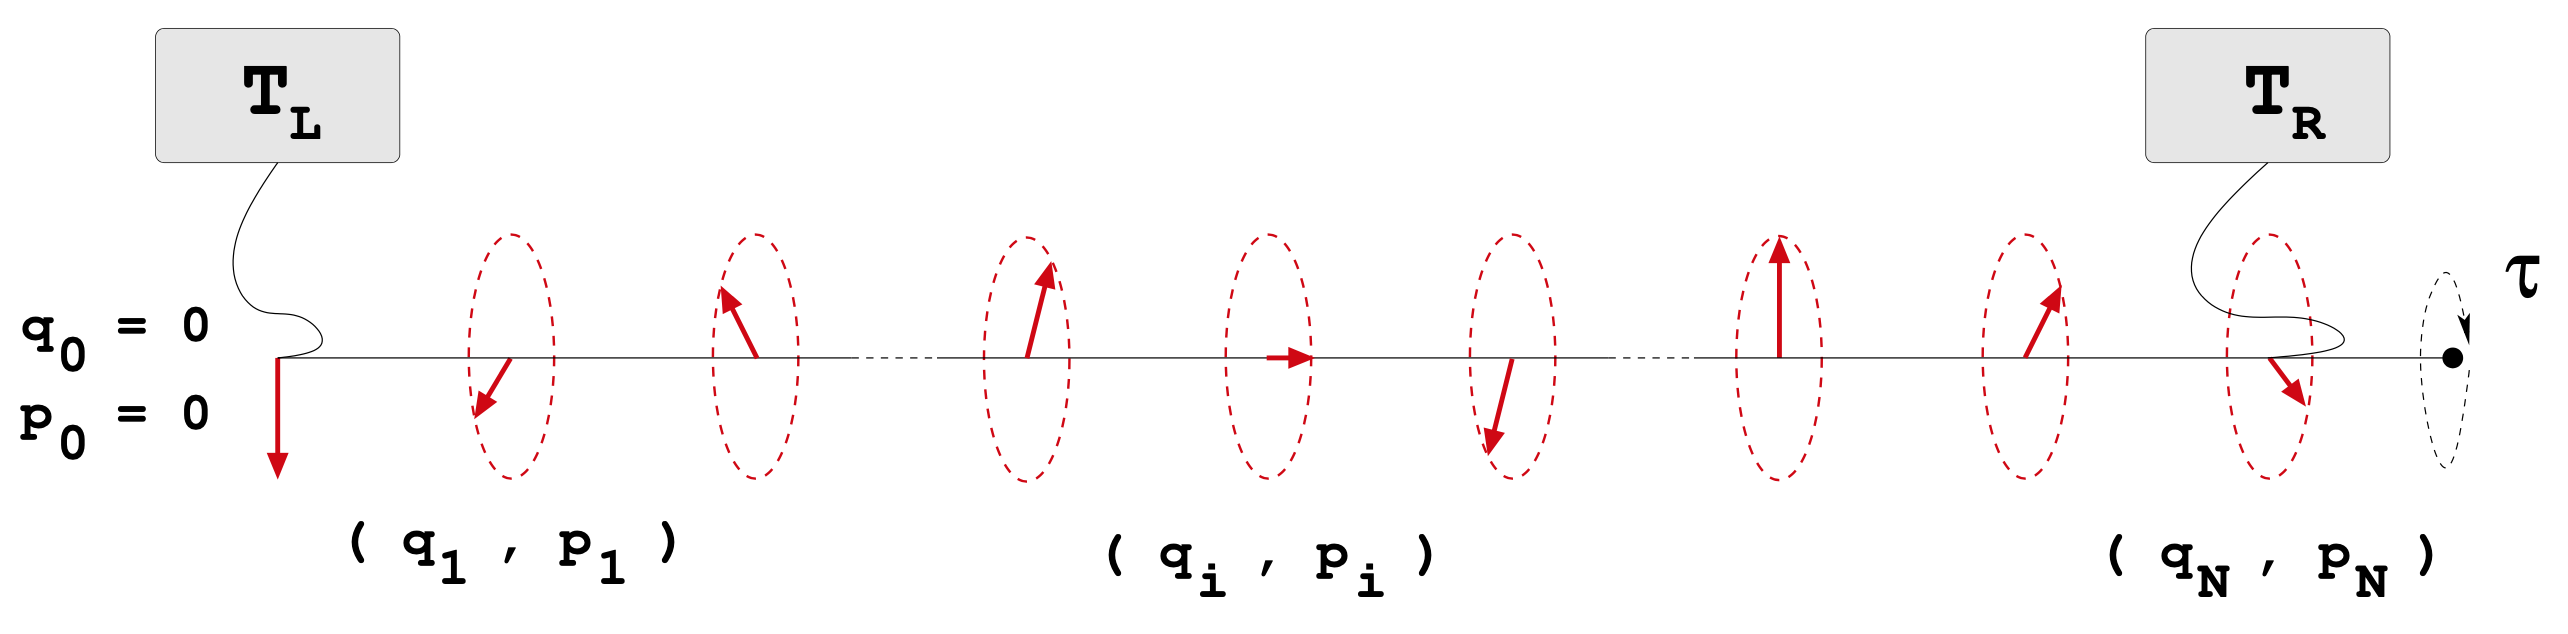
\includegraphics[scale=0.24]{images/rotor_chain.png}
    \end{figure}

    Source : Alessandra Iacobucci, Nonequilibrium stationary states of
    rotor and oscillator chains~\cite{Iacobucci_2011}.

\end{frame}

\begin{frame}

    \frametitle{Modèle - Thermostat de Langevin}

    Un thermostat de Langevin agit comme un bain chauffant.
    Un objet immergé dans un tel bain est
    frappé rapidement par des petites particules, ce qui
    induit un changement de la vitesse (température) de l'objet.
    Par ailleurs, lorsqu'il se déplace, l'objet est restreint
    par les particules du bain, ce qui réduit sa vitesse.

    Ce comportement est un type de fluctuation-dissipation. C'est
    exactement ce qu'on observe dans le mouvement brownien. Un
    grain de pollen immergé dans l'eau, par exemple, est
    poussé par l'agitation thermique des molécules de l'eau, et,
    simultanément, le grain est restreint par la viscosité de l'eau.

\end{frame}

\begin{frame}

    \frametitle{Modèle - Thermostat de Langevin}

    Mathématiquement, un thermostat de Langevin s'exprime alors
    comme la somme de ces 2 forces : celle de la dissipation et celle
    de la fluctuation. Son effet sur le mouvement cinétique est
    donné par
    %
    \[dp = - \gamma p dt + \sigma dW_t,\]
    %
    où $W_t$ est un processus de Wiener standard, et $\sigma$ et $\gamma$
    sont liés par la relation de fluctuation-dissipation :
    \[\sigma^2 = 2 \gamma mkT\]
    %
    Avec $m = k = 1$, on a donc
    \[dp = - \gamma p dt + \sqrt{2 \gamma T_L} dW_t\]

    % The damping factor and the randomforce combine to give the correct canonical ensemble.

\end{frame}


%\begin{frame}
%
%    \frametitle{Modèle - Forçage}
%
%    C'est du type non gradient...
%
%    \colorbox{green}{Ça modelise quoi ?}
%
%    %     % It is precisely because the perturbation is not of gradient type that
%    %    % some particle flux can appear in the steady-state.
%
%\end{frame}


\begin{frame}

    \frametitle{Modèle - Hamiltonien}

    Avec le potentiel $V = \sum_i 1 - \cos(q_i - q_{i-1})$ on
    a le hamiltonien
    %
    \[H(q,p) = \sum_{i=1}^N \left[ \frac{p_i^2}{2}
             + (1 - \cos (q_i - q_{i-1})) \right]\]
    %
    Et les equations de Hamilton,
    \begin{align*}
        dq_i &= p_i dt, \\
        dp_i &= (\sin(q_{i+1} - q_i) - \sin(q_i - q_{i-1}))dt
    \end{align*}


\end{frame}




\begin{frame}

    \frametitle{Modèle - Équations d'évolution}

    En combinant les équations de Hamilton, le forçage $F$, et des
    thermostats de Langevin à gauche et à droite de la chaîne,
    on en tire les équations d'évolution du système :
    %
    \begin{align*}
        dq_i &= p_i dt, \\
        dp_i &= (\sin(q_{i+1} - q_i) - \sin(q_i - q_{i-1}))dt \quad (i \neq 1, N), \\
        dp_1 &= (\sin(q_2 - q_1) - \sin(q_1))dt - \gamma p_1 dt + \sqrt{2 \gamma T_L} dW_t^1, \\
        dp_N &= (F - \sin(q_N - q_{N-1})) dt - \gamma p_N dt + \sqrt{2 \gamma T_R} dW_t^N
    \end{align*}

%    \label{eq:dynamique}

    % Ce qui est précisément la dynamique \eqref{eq:dynamique}.

\end{frame}


